\documentclass[12pt]{article}
\usepackage{amsmath}
\usepackage[linesnumbered,ruled]{algorithm2e}
\usepackage[noend]{algpseudocode}
\usepackage{graphicx}
\usepackage{hyperref}
\usepackage{tikz,forest}
\usetikzlibrary{arrows.meta}
\usepackage{forest}
\usepackage{adjustbox}
\usepackage{skmath}
\usepackage{inputenc}
\usepackage{amsmath,amsthm,amssymb}
 \usepackage{tabu}
 \usepackage{graphicx}
\usepackage{wrapfig}
\graphicspath{ {images/} }
\usepackage{tcolorbox}
\newtheorem*{remark}{Remark}

\makeatletter
\def\BState{\State\hskip-\ALG@thistlm}
\makeatother

\forestset{
    .style={
        for tree={
            base=bottom,
            child anchor=north,
            align=center,
            s sep+=1cm,
    straight edge/.style={
        edge path={\noexpand\path[\forestoption{edge},thick,-{Latex}] 
        (!u.parent anchor) -- (.child anchor);}
    },
    if n children={0}
        {tier=word, draw, thick, rectangle}
        {draw, diamond, thick, aspect=2},
    if n=1{%
        edge path={\noexpand\path[\forestoption{edge},thick,-{Latex}] 
        (!u.parent anchor) -| (.child anchor) node[pos=.2, above] {Y};}
        }{
        edge path={\noexpand\path[\forestoption{edge},thick,-{Latex}] 
        (!u.parent anchor) -| (.child anchor) node[pos=.2, above] {N};}
        }
        }
    }
}


\begin{document}
\noindent
{\large{ \textbf{Game Theory} }}\\

\noindent
\textsl{1. Single-move games }\\

\noindent
\textsl{1.1 Game}
\begin{itemize}
\item A single-move game is defined by \textbf{3} components:

\begin{itemize}
\item \textbf{Player/agent} who makes decisions. We mostly look at 2 players games
\item \textbf{Actions} that the players can choose
\item A \textbf{payoff function} that gives the utility to each player for each combination of actions chosen by all players. A payoff function can be represented by a matrix, called strategic form/normal form. For example: \\
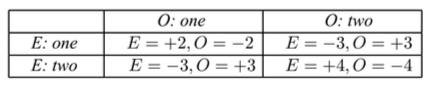
\includegraphics[scale=0.5]{p1}
\end{itemize}

\item Each player adopts and executes a \textbf{strategy}.
 \begin{itemize}
 \item A \textbf{pure strategy} is a deterministic action
 \item A \textbf{mixed strategy} is a randomized policy that selects an action based on a probability distribution 
 \item Strategy $s$ \textbf{strictly dominates} strategy $s'$ if outcome for $s$ is better than outcome for $s'$, for every choices of other players (that is, independent of other's choices)
  \begin{itemize}
  \item If iterated elimination of strictly dominated strategies results in one strategy for each player we have found a unique equilibrium
  \item Order of elimination does not matter 
  \end{itemize}
 \item Strategy $s$ \textbf{weakly dominates} strategy $s'$ if $s$ is better than $s'$ for at least one strategy profile and no worse on any other.
   \begin{itemize}
  \item  If we also eliminates weakly dominated strategies and end up with one strategy for each player, we have also found an equilibrium, but there may be other equilibrium that we did not found.
  \end{itemize}
  
  
 \item If a strategy is better than all other strategies independently of the strategies chosen
by the other players we call the strategy a \textbf{dominant strategy}.

 \end{itemize}
 
 \item A \textbf{strategy profile} is an assignment of strategy to each player. For example: for player $p$, plays $[one: 0.5; two: 0.5]$; for player $q$, plays $[one: 0.3; two: 0.7]$

\item Given a strategy profile, an \textbf{outcome} is a numeric result for \textbf{each player} that obtains from a \textbf{specific combination} of player's strategies. Every combination of strategies (one for each player) is an outcome of the game. A primary purpose of game theory is to determine which outcomes are stable, in the sense of being Nash equilibria.

\item A \textbf{solution} is a strategy profile where each player adopts a rational strategy
 \begin{itemize}
 \item When the player is the environment, rational means to maximize expected utility
 \end{itemize}
\end{itemize}

\noindent
\textsl{1.2 Equilibrium}

\begin{itemize}
\item A strategy profile forms an \textbf{equilibrium} if no players can benefit from switching strategies, given that every other players stick to the same strategies
\begin{itemize}
\item An equilibrium is a \textbf{local optimal}
\end{itemize}
\item The combination of each player's dominant strategy, if each has one, is called \textbf{dominant strategy equilibrium}
\item Equilibrium is also called \textbf{Nash equilibrium}
\item Algorithm of \textbf{finding pure strategy Nash equilibrium}:
\begin{itemize}
\item For each column, mark cell if it has the maximum payoff for the row player
\item For each row, mark cell if it has the maximum payoff for the column player
\item Cells with both row and column marks are pure Nash equilibrium
\end{itemize}

\end{itemize}

\noindent
\textsl{1.3 Pareto Optimal}
\begin{itemize}
\item An outcome is \textbf{Pareto optimal} if there is no other outcomes that all players would prefer
\item An outcome is \textbf{Pareto dominated} by other outcome if all players would prefer the other outcome
\begin{itemize}
\item Some other outcomes would make at least one player better off without making other players worst
\end{itemize}
\item If an outcome is not Pareto dominated, then it is Pareto optimal
\end{itemize}

\noindent
\textsl{1.4 Mixed strategies}

\begin{itemize}
\item A game may also have mixed strategies Nash equilibrium\\

 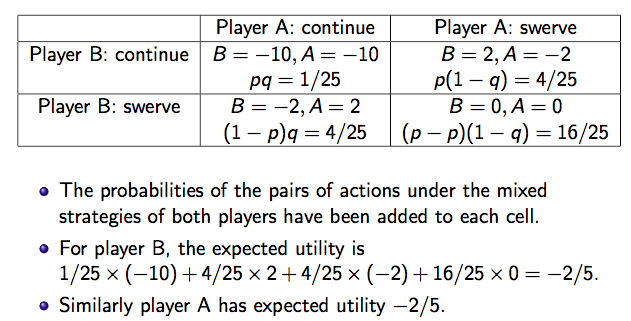
\includegraphics[scale=0.5]{p2}
\begin{itemize}
\item The algorithm works by finding a mixture for one player where the other player becomes indifferent to the choice and doing that for both players. However, this algorithm does not always work if there is no mixture that the other player becomes indifferent. For example, when a player has a dominant strategy thus cannot be indifferent to the choices
\end{itemize}

\item \textbf{Finding optimal mixed strategy for a two-player zero sum game: Minimax theorem }
\begin{tcolorbox}
$\operatorname*{arg\,max}_x \operatorname*{arg\,min}_y x^TAy = \operatorname*{arg\,min}_y \operatorname*{arg\,max}_x x^TAy = v$ 
\end{tcolorbox}
\begin{itemize}
\item $v$ is the value of the game/expected outcome for one player, $-v$ for the other player (zero-sum game)
\item The minmax strategy for O (minimizer) (and maxmin strategy for E(maximizer)) gives a Nash equilibrium for the game
\item Who goes first does not matter
\item If the first player plays the corresponding mixed strategy, the second player can play a pure strategy to get the game value, but cannot do better with any other strategy
\item Find the corresponding $x$ and $v$ by solving linear programming: 

$ \forall j$, maximize $v$ with $v \leq \sum_{x}^{} a_{ij} \times x_i$, and $\sum_{}^{} x_i = 1(x_i \geq 0) $.
\begin{itemize}
\item $a_{j}$ is the $j$-th row of $A$, $a_{ij}$ is the element in $j$-th row of $A$.
\end{itemize}
\end{itemize}

\end{itemize}

\end{document}